\documentclass{article}[18pt]
\usepackage{../../../../format}
\lhead{Networks and Systems - Security}


\begin{document}
\begin{center}
\underline{\huge Network \& Web Security}
\end{center}
\section{Border Gateway Protocol}
\begin{itemize}
	\item What if you want to take down a big chunk (or all) of the internet
	\item BGP trusts all route announcements sent by its peers
	\item Announcing a shorter route through a blank page would cause chaos
\end{itemize}
\section{Router Security}
Security Features:
\begin{itemize}
	\item Firewalls (also stateful packet inspection)
	\item VPN Handling
	\begin{itemize}
		\item Confidentiality via encryption
		\item Authentication
		\item Message integrity (detect instances of tampering with transmitted messages)
	\end{itemize}
\end{itemize}
NAT
\begin{itemize}
	\item Allows a LAN to appear under a single machine with a single IP address (e.g. limited IPv4 address space)
	\item Breaks the end to end communication model
	\item NATs don't make internal network topology secure
\end{itemize}
\section{Telnet, SSH, Netcat and FTP}
\begin{itemize}
	\item Telnet is a very old protocol that should not be used any more
	\begin{itemize}
		\item All data is sent unencrypted in plain text
		\item Easy to capture passwords using a packet sniffer
		\item Subject to MITM attacks
	\end{itemize}
	\item Telnet replaced by SSH
	\begin{itemize}
		\item Strong encryption with public key authentication ensuring remote computer is who it claims to be
	\end{itemize}
	\item FTP is also obsolete (except insensitive data)
	\begin{itemize}
		\item Sends login and password in clear text vulnerable to sniffing attacks
		\item Do FTP over SSH (SFTP)
		\item Check FTP server path is pointing to sensible location
	\end{itemize}
\end{itemize}
\section{ARP Vulnerabilities and NDP}
\begin{itemize}
	\item Maps Internet Protocol (IPv4, 32bits) address to physical machine (MAC address, 48bits)
	\item Vulnerable to
	\begin{itemize}
		\item ARP Spoofing
		\begin{itemize}
			\item Steal sensitive information
			\item DoS, MITM, Session-Hijacking
		\end{itemize}
		\item MAC Flooding
		\item MAC Duplicating
	\end{itemize}
	\item Still widely used, but replaced by NDP for IPv6
\end{itemize}
\section{NDP}
\begin{itemize}
	\item Also resolved network layer (IP) and link layer like ARP, but for IPv6
	\item Secure Neighbour Discovery (SEND) security extension
	\begin{itemize}
		\item Cryptographically generated addresses ensure that the claimed source of an NDP message is the owner of the claimed address
	\end{itemize}
	\item Offers lots of improvements over IPv4 equivalent protocols. Some:
	\begin{itemize}
		\item Better router discovery
		\item More robust to failures where neighbours become unreachable
	\end{itemize}
	\item But still far from perfect
	\begin{itemize}
		\item Still vulnerable to MITM via:
		\begin{itemize}
			\item Spoofed ICMPv6 neighbourhood router advertisement
			\item Rogue DHCPv6 Servers, and other approaches
		\end{itemize}
		\item Vulnerable to DoS by flooding and many others
	\end{itemize}
\end{itemize}
\section{IP Spoofing}
\begin{itemize}
	\item Changing the source IP of a packet with a fake IP address to hide the identify of the sender
	\item The victim thinks he's talking to his friend, but actually he's talking to the hacker
	\item Protection
	\begin{itemize}
		\item Authentication protocol
		\item Encrypted sessions
		\item Access control lists (ACLs)
		\item Filtering of traffic
		\item Proper router configuration
	\end{itemize}
\end{itemize}
\section{Distributed Denial of Service (DDoS)}
This is very difficult to protect against
\begin{center}
	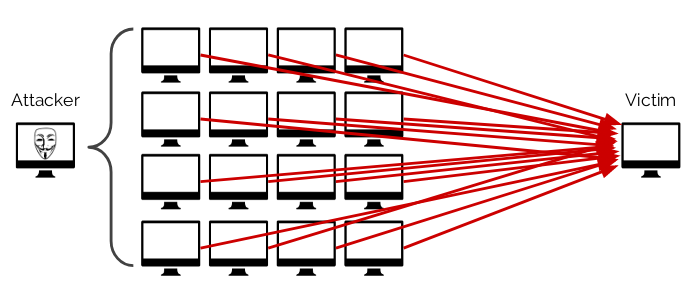
\includegraphics[scale=0.7]{DDoS}
\end{center}
\section{Wiretapping}
A passive splice tap can be placed in a copper cable in order to read all the data passing along the cable
\section{Cross-Site Scripting (XSS)}
\begin{center}
	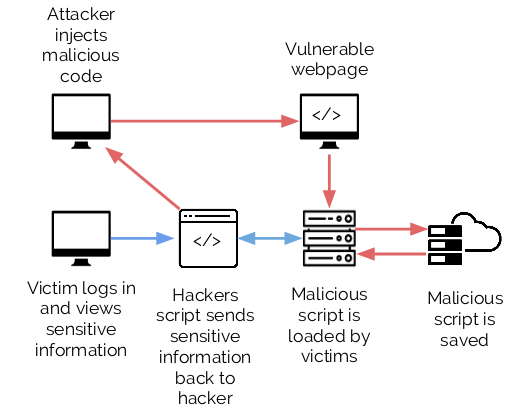
\includegraphics[scale=0.7]{XSS}
\end{center}
Protection
\begin{itemize}
	\item Whitelisting - only allow valid inputs on server
	\item HTML escaping
	\item Sanitization
	\item Blacklisting - quite fragile and not very good
\end{itemize}
\section{Cookies}
Credential tokens:
\begin{itemize}
	\item Held in local browsing session
	\item Identify you to a remote web server
	\item Remember states
	\begin{itemize}
		\item Shopping cart
		\item Browsing history
		\item Data in form fields
	\end{itemize}
	\item Common target for hackers
\end{itemize}
\end{document}